\chapter{Electron/pion and electron/muon classifiers based on artificial neural networks}\label{appendix:clasifiers}

The rejection of background components where the DC track identified as electron or positron in fact corresponds to either a poorly recorded charged pion or to a muon from a $\pi^{\pm}\to\mu^{\pm}\bar{\nu}_{\mu}$ decay, presented in~\sref{sec:pimu_rejection}, is based on artificial neural networks. Other machine learning solution were considered as well, such as Boosted Decision Trees and the $k$-Nearest Neighbors algorithm (all in their implementation from the TMVA software package~\cite{Hocker:2007ht}). However, as the classification problem considered in this case is rather uncomplicated, all of these methods exhibited comparable performance, with the output from neural networks allowing for a combination of the two ($e$/$\pi$ and $e/\mu$) classifiers' results most convenient to design a background rejection cut.

The employed ANN-s were simple feed-forward networks with each with five inputs, a single 10-neuron hidden layer and a single output. The input variables were not subject to any preparatory transformations. The two first input variables used are based on the different longitudinal structure of electromagnetic showers from $e^{\pm}$ and from $\pi^{\pm}$/$\mu^{\pm}$ in the KLOE calorimeter. First variable is defined as normalized difference of energies deposited in the first and second calorimeter layers with non-zero recorded energy:
\[ \Delta E_{12} = \frac{E_{dep}^{1st\:layer} - E_{dep}^{2nd\:layer}}{E_{dep}^{1st\:layer} + E_{dep}^{2nd\:layer}}. \]  

\begin{figure}[h!]
  \centering
  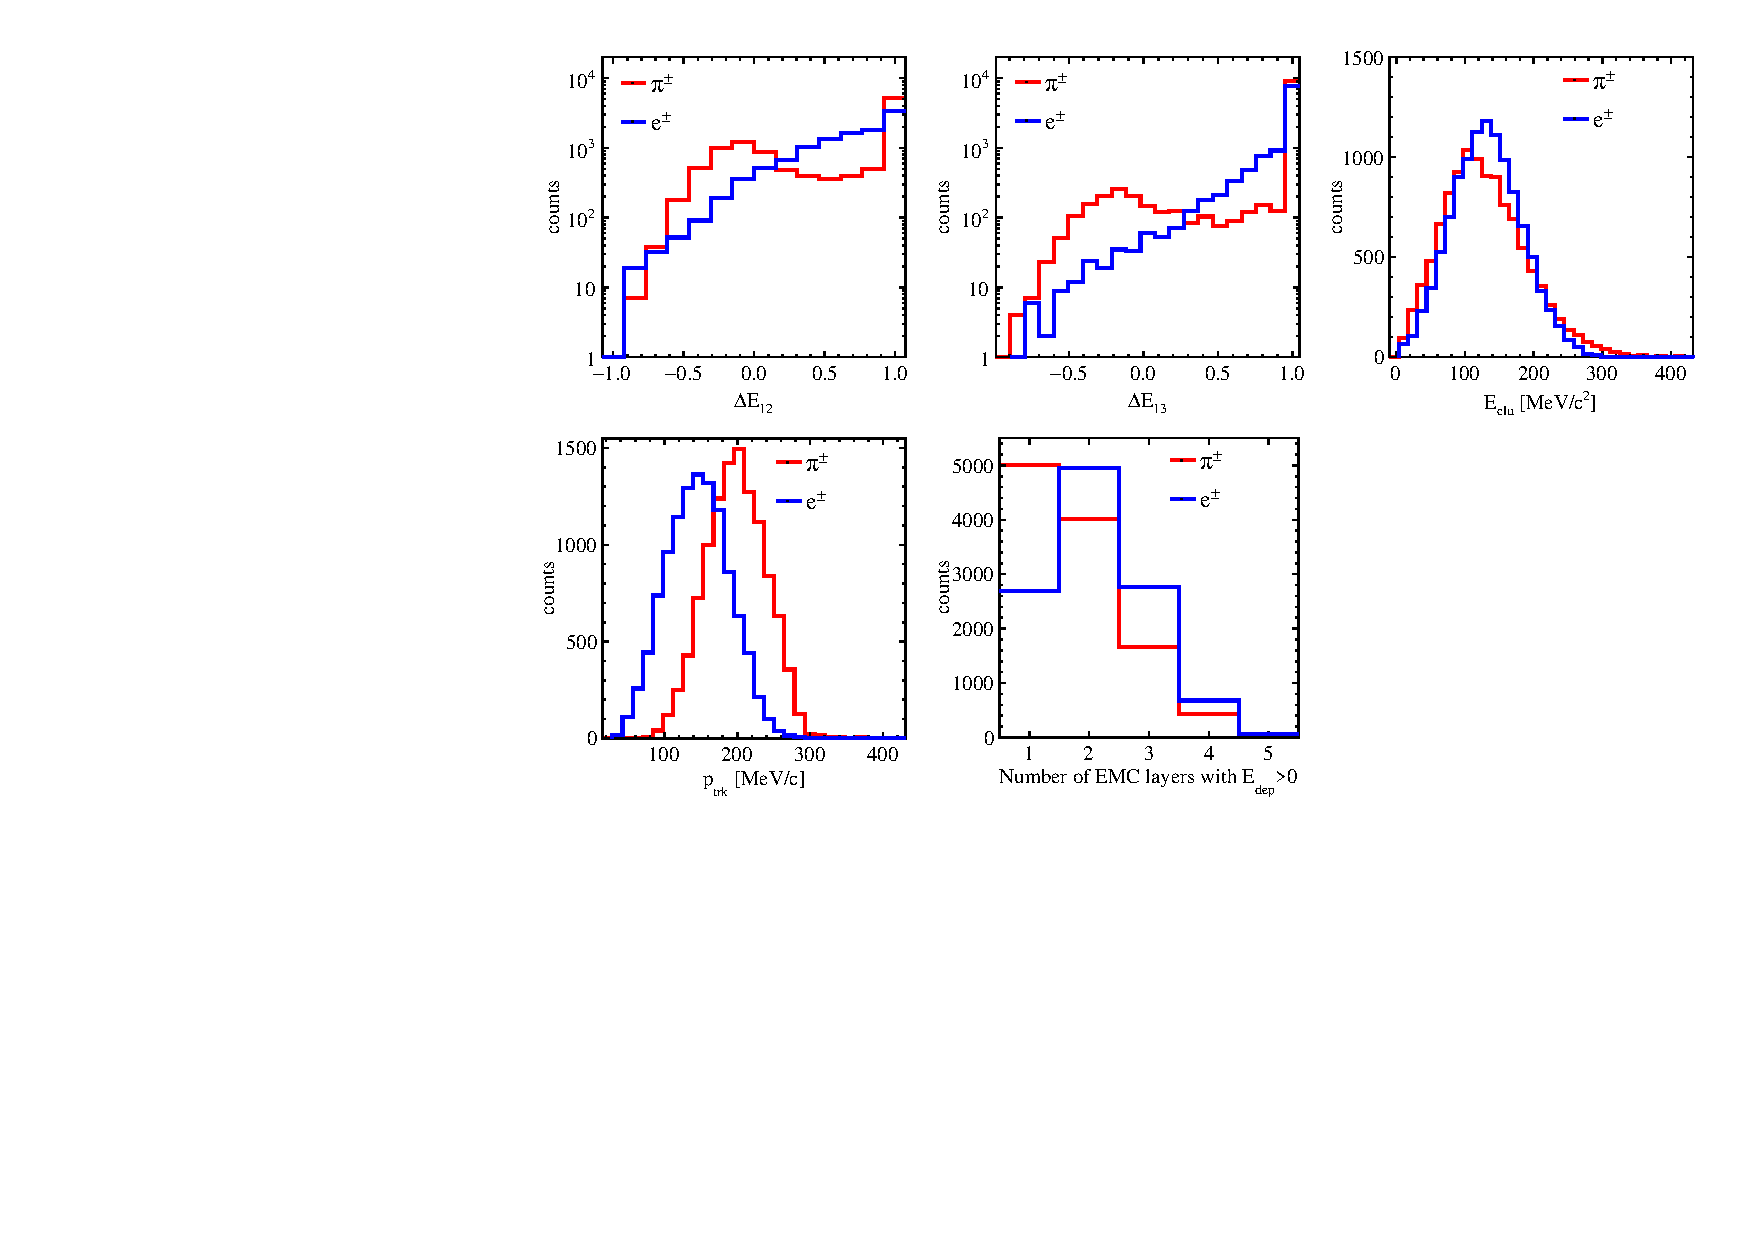
\includegraphics[width=1.0\textwidth]{Chapter7_analysis_kloe/img/csps/inputs_pi}
  \caption{Distributions of five variables characterizing the EMC cluster identified as coming from a lepton and its associated DC track, used as input for the $e$/$\pi$ classifier. The distributions were obtained with a $\Kl\to\pi e\nu$ data sample used for training of the neural network.}\label{fig:mva_inputs_epi}
\end{figure}

Similarly, the second input variable is a relative difference between energies deposited in the first and third active EMC layers:
\[ \Delta E_{13} = \frac{E_{dep}^{1st\:layer} - E_{dep}^{3rd\:layer}}{E_{dep}^{1st\:layer} + E_{dep}^{3rd\:layer}}. \]  
As visible in Figures~\ref{fig:mva_inputs_epi} and~\ref{fig:mva_inputs_emu}, distributions of $\Delta E_{12}$ and $\Delta E_{13}$ are closer to unity for electrons/positrons, in accordance with the large deposition of energy at the first interactions expected from these particles. In a large number of events, however, the energy deposited in one or both of the subsequent layers is zero e.g.\ due to limited efficiency of the calorimeter for small energy deposits, which results in the values of normalized differences equal to unity. As this effect occurs for all considered types of particles alike, discrimination in such cases must be based on other input. Therefore, another input to the classifiers is constituted by the number of EMC layers which recorded a non-zero energy deposit. As shown in the last panel of Figures~\ref{fig:mva_inputs_epi} and~\ref{fig:mva_inputs_emu}, most electrons activate at least two layers of the calorimeter whereas both $\pi^{\pm}$ and $\mu^{\pm}$ tend to often deposit a registerable energy amount in a single layer only. Finally, the last two variables used as input of the classifiers are the particle momentum estimated with the DC track and total energy deposited in the EMC cluster associated to that track. As both these quantities are measured independently, their relative values allow for a good discrimination between electrons/positrons and heavier particles. Distributions of all five input variables compared between electrons/positrons and charged pions and muons are presented in Figures~\ref{fig:mva_inputs_epi} and~\ref{fig:mva_inputs_emu}, respectively.

\begin{figure}[h!]
  \centering
  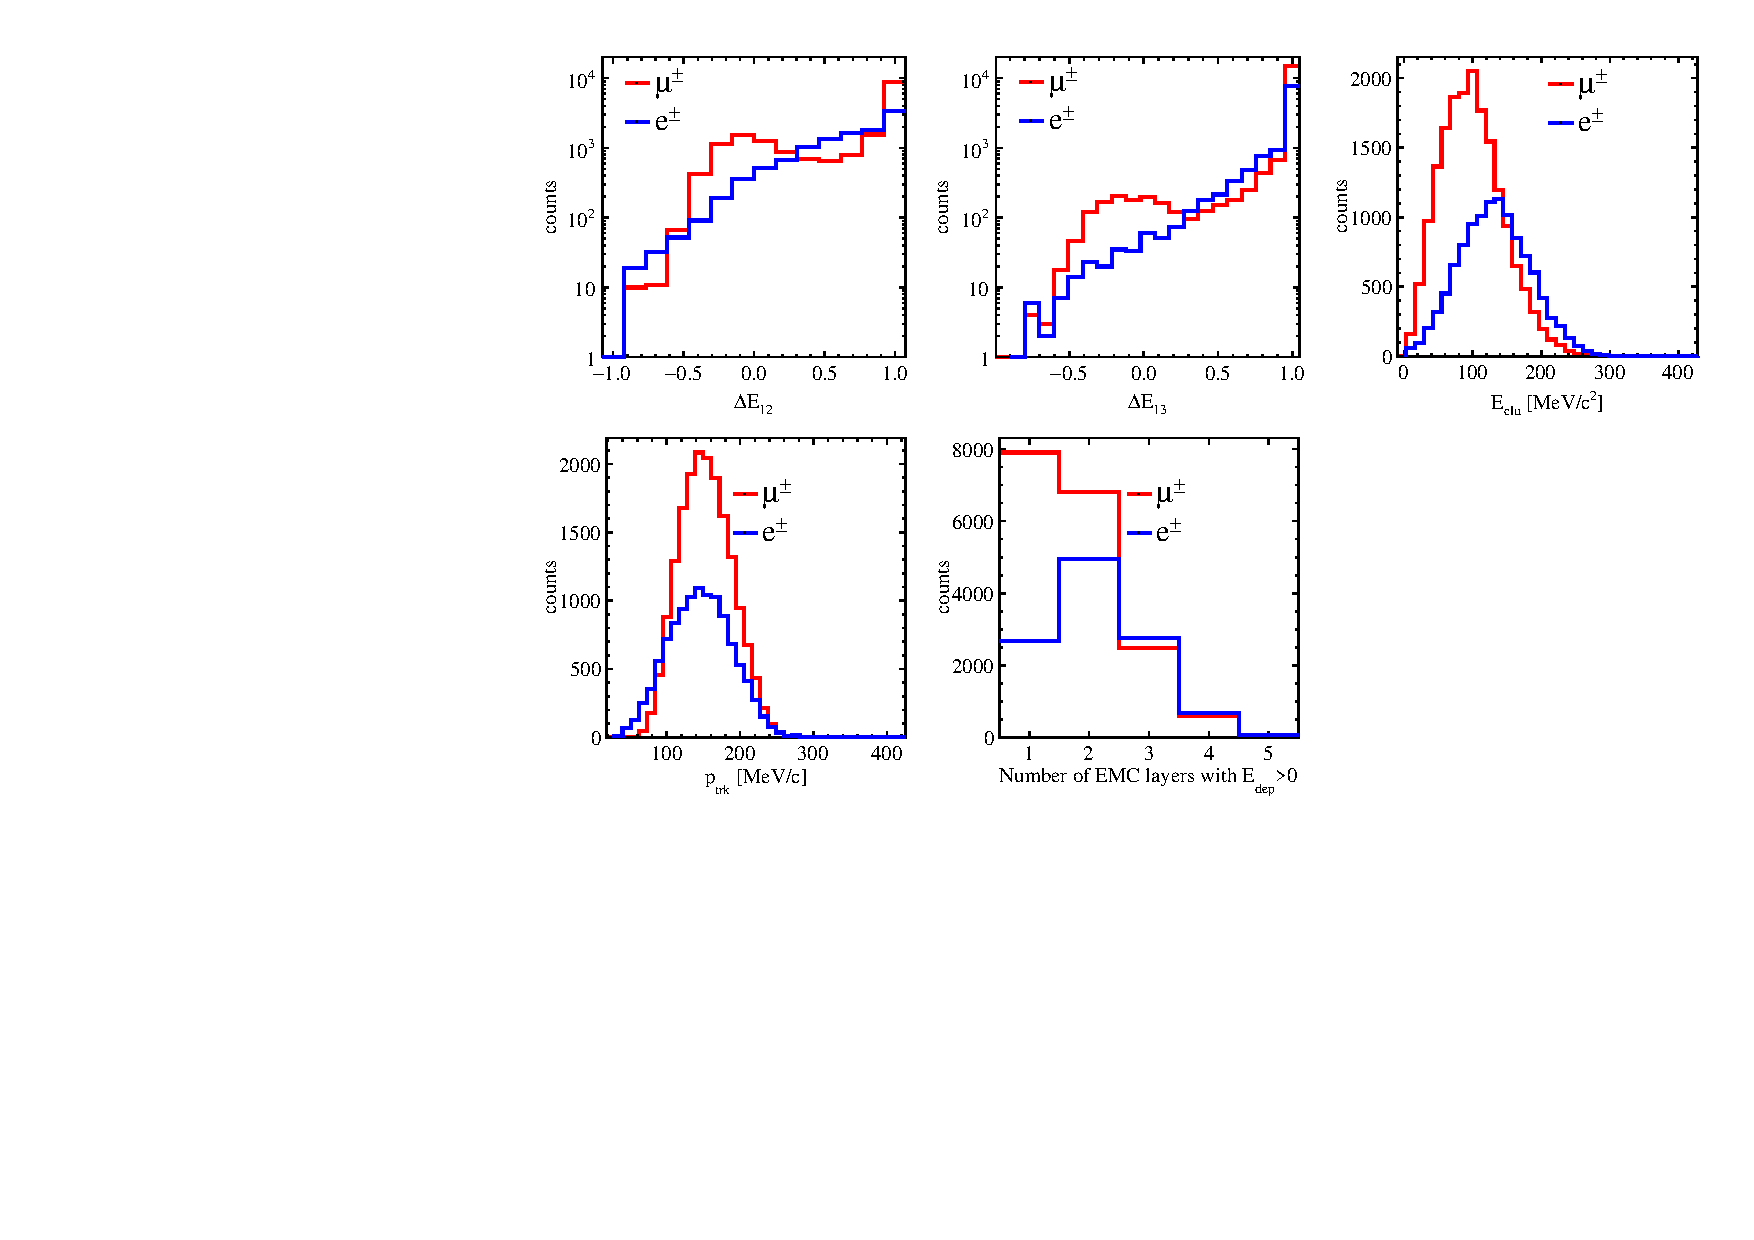
\includegraphics[width=1.0\textwidth]{Chapter7_analysis_kloe/img/csps/inputs_mu}
  \caption{Distributions of five variables characterizing the EMC cluster identified as coming from a lepton and its associated DC track, used as input for the $e$/$\mu$ classifier. The distributions were obtained with a $\Kl\to\pi\mu\nu$ data sample used for training of the neural network.}\label{fig:mva_inputs_emu}
\end{figure}


%%%Local Variables:
%%% TeX-master: "../main"
%%% End: